\documentclass{beamer}

\usepackage[utf8]{inputenc}
\usepackage[ngerman]{babel}
\usepackage{default}
\usepackage{graphicx}

\usetheme{Goettingen}
\usecolortheme{seagull}

\author{Daniel Pollack}
\title{Bachelorpräsentation}
\institute{Bauhaus-Universität Weimar\\Lehrstuhl: Human-Computer Interaction}


\begin{document}
\begin{frame}
 \titlepage
\end{frame}

\begin{frame}
 \frametitle{Inhalt}
 \tableofcontents
\end{frame}

\begin{frame}
 \section{Komponenten}
 \frametitle{Komponenten}
\end{frame}

\begin{frame}
 \section{PC $\leftrightarrow$ Arduino Kommunikation}
 \frametitle{PC $\leftrightarrow$ Arduino Kommunikation}
 \begin{block}{Stand}
  weitestgehend implementiert
 \end{block}
 \begin{block}{ToDo}
  automatische Erkennung und Verbindung
  Geschwindigkeitstest
 \end{block}
\end{frame}

\begin{frame}
 \section{Plot}
 \frametitle{Plot}
 \begin{block}{Plot}
  Plotbibliothek gefunden: Oxyplot
  \begin{itemize}
  \item einfache Verwendung
  \item mangelnde Dokumentation
  \item $>$ 1 Plot pro Oberfläche verursachen zufällige Abstürze
 \end{itemize}
 \end{block}
\end{frame}

\begin{frame}
\section{Platine}
\frametitle{Platine}
  \begin{block}{Erstellung einer Testplatine}
  Erarbeitung läuft
  \end{block}
\end{frame}
\begin{frame}
  \frametitle{Ursprüngliches Design}
  \begin{figure}
    \centering
    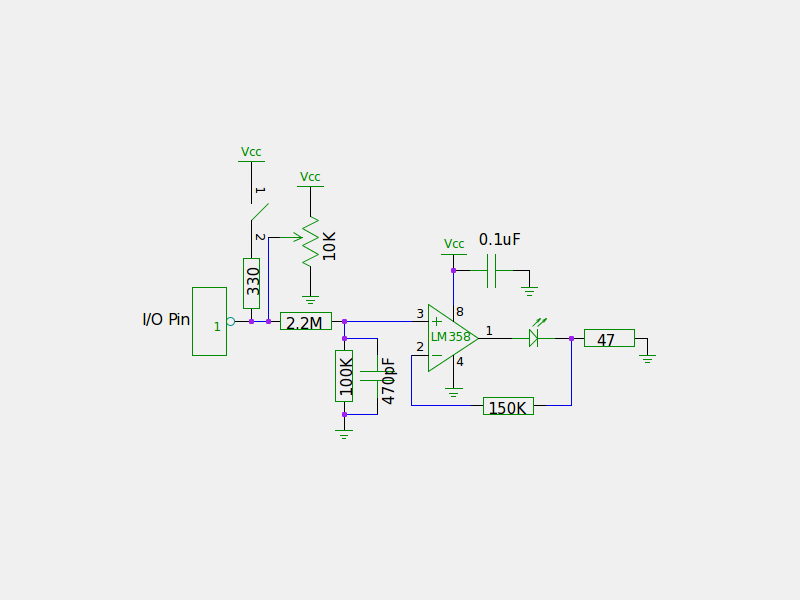
\includegraphics[width=\textwidth,keepaspectratio]{./pics/Board1.png}
  \end{figure}
\end{frame}
\begin{frame}
  \frametitle{Aktuelles Design}
  \begin{figure}
    \centering
    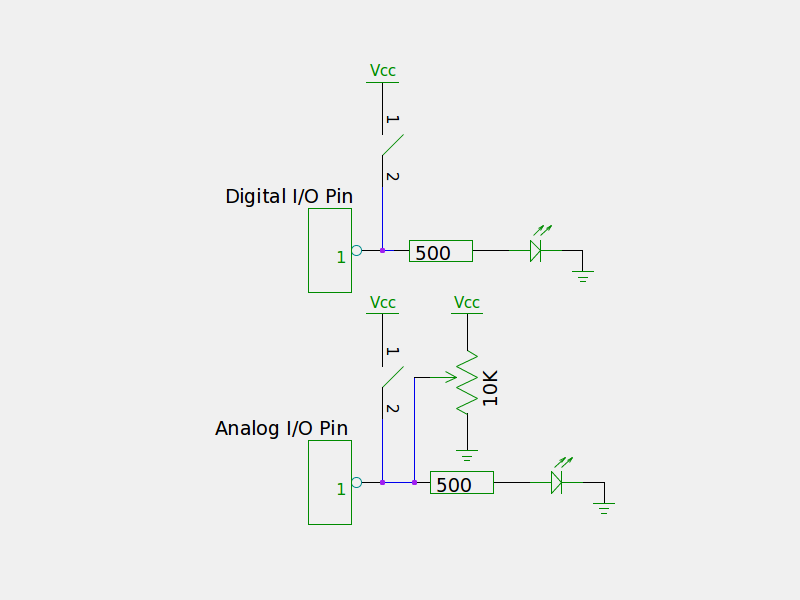
\includegraphics[width=\textwidth,keepaspectratio]{./pics/Board2.png}
  \end{figure}
\end{frame}

\begin{frame}
 \section{Sonstiges}
 \begin{block}{Sonstiges}
  gestern (1. Juni 2015) Treffen mit dem Datenloggingexperten des Max-Plank Institutes
  \begin{itemize}
  \item Erklärung der Arbeitsabläufe
  \item Erläuterung der eingesetzten Technik und derren Bedienung
  \end{itemize}
  \end{block}
\end{frame}

\end{document}
